\documentclass{article}
\usepackage[utf8]{inputenc}
\usepackage{datetime}
\usepackage{enumerate}
\usepackage{textcomp}
\usepackage{amsmath}
\usepackage{amssymb}
\usepackage[edges]{forest}
\usepackage{tikz}
\usetikzlibrary{shapes, backgrounds, automata, positioning, arrows}
\usetikzlibrary{arrows}
\usepackage{listings}
\usetikzlibrary{graphs}

\usepackage{titlesec}
\newcommand{\sectionbreak}{\clearpage}

\title{\bf \Large HW 1}
\author{Xinhao Luo} 
\date{\today}

\def\math#1{$#1$}

\setlength{\textheight}{8.5in}
\setlength{\textwidth}{6.5in}
\setlength{\oddsidemargin}{0in}
\setlength{\evensidemargin}{0in}
\voffset0.0in

\begin{document}

\maketitle

\section{Problem 1}

\begin{itemize}
    \item Answer: \math{2^n}
    \item Prove By Induction
        \begin{itemize}
            \item Observe the program, we have: \math{T(n) = 1 + (T(0) + T(1) + T(2) + T(3) + ... + T(n-1))}
            \item [Base Case] \math{T(0) = 1 = 2^0}
            \item [Induction Step] Assume \math{T(n) = 2^n}, Prove \math{T(n+1) = 2^{n+1}}, Let: 
                \begin{itemize}
                    \item 
                        \begin{equation}
                            \begin{split}
                                S &= 2^0 + 2^1 + 2^2 + ... + 2^n \\
                                2S &= 2^1 + 2^2 + 2^3 + ... + 2^{n+1} \\
                                2S - S &= 2^1 - 2^1 + 2^2 - 2^2 + 2^3 - 2^3 + ... + 2^{n+1} - 2^0 \\
                                S &= 2^{n+1} - 1
                            \end{split}
                        \end{equation}
                    \item We have \math{T(n+1) = 1 + 2^{n+1} - 1 = 2^{n+1}}
                \end{itemize}
        \end{itemize}
    \item Proved \math{T(n) = 2^n}
\end{itemize}

\section{Problem 2}

\begin{itemize}
    \item It is observed that \math{T(n) = n + (n-1) + (n-2) + (n-3) + ... + 0 = \frac{n^2+n}{2}}
    \item []
        \begin{itemize}
            \item [Base Case] \math{T(0) = 0}
            \item [Induction Step] Assume \math{T(n) = \frac{n^2+n}{2}}, prove \math{T(n+1) = \frac{(n+1)^2 + (n+1)}{2}} \\
                \begin{equation}
                    \begin{split}
        T(n+1) &= 1 + 2 + 3 +... + (n + 1) \\
        &= \frac{n^2+n}{2} + n + 1 \\
        &= \frac{n^2 + n + 2n + 2}{2} \\
        &= \frac{(n+1)^2+(n+1)}{2}
                    \end{split}
                \end{equation}
        \end{itemize}
    \item Proved that \math{T(n) = (n^2 + n) / 2}
\end{itemize}

\section{Problem 3}
\begin{enumerate}[a)]
    \item Prove by Induction
        \begin{itemize}
            \item [Base Case] when \math{u = 0}, Sum of \math{d(u) = 0 = 2|E|}
            \item [Induction Step] Assume claim is true for any graph with \math{u} nodes, prove it is still applied for \math{u + 1}. \\
            The number of degree for \math{u + 1} is \math{2(n + 1) = 2n + 2} \\ 
            Every time we have a new edge, it will connect two vertices, and each vertices will increase degree by 1. In total, an edge increase degree by 2, so that degrees will be equal to 2x edges
        \end{itemize}
    \item Prove by contradiction
            \begin{itemize}
                \item Assume there are odd number of vertices has odd degrees
                \item The rest of the nodes will be even degrees for sure.
                \item An odd number times an odd number will always be odd, and either even number of an odd number times and odd number, the result will be even
                \item The total degree will be an odd number plus a even number, which will be odd number
                \item the total degree of a graph will always a even number, which contradicted with the previous conclusion
                \item [conclusion] The original statement must be true: even number of vertices has odd degrees
            \end{itemize}
    \item 
        \begin{enumerate}[a)]
            \item No, Prove by counter example \\ 

            \begin{tikzpicture}[>=stealth, every node/.style={circle, draw, minimum size=0.75cm}]
                \graph [tree layout, grow=down, fresh nodes, level distance=0.5in, sibling distance=0.5in]
                {
                    1 -> { 2} 
                };
            \end{tikzpicture} \\
            The indegree is 1 here.
            \item No, Prove by counter example \\
            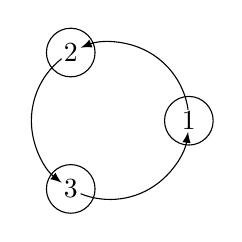
\begin{tikzpicture}
                \def \n {3}
                \def \radius {1cm}
                \def \margin {8} % margin in angles, depends on the radius
                
                \foreach \s in {1,...,\n}
                {
                  \node[draw, circle] at ({360/\n * (\s - 1)}:\radius) {$\s$};
                  \draw[->, >=latex] ({360/\n * (\s - 1)+\margin}:\radius) 
                    arc ({360/\n * (\s - 1)+\margin}:{360/\n * (\s)-\margin}:\radius);
                }
                \end{tikzpicture} \\
                Each node has only one indegree, but the total number of vertices is odd as well
        \end{enumerate}
\end{enumerate}

\section{Problem 4}
\begin{itemize}
    \item [] \textbf{Algorithm}
        \begin{enumerate}[Step 1]
            \item For each node in graph \math{G_1}, use BFS to find the shortest path to node \math{s}, and save the distance into a Hashtable (with O(1) average access time). Use BFS and find shortest distance and store for graph \math{G_2} repectively.
            \item For each edge \math{E_1}, we may find its distance \math{D_1} to \math{s}, and distance \math{D_2} to \math{t} in \math{G_1}. The total shortest distance of given edge \math{D} can be calculated as following: \\
            \begin{equation}
                D = D_1 + D_2 + 1
            \end{equation} \\ 
            We may keep replace \math{D} if current edge in \math{E'} is smaller than the previous one so that we will always have the smallest path
            \item We compared the shortest distance \math{D} we have from previous step, with the given number.  \textbf{Return true if same, false otherwise}
        \end{enumerate}
    % \item [] \textbf{Time Complexity}
    %     \begin{enumerate}[Step 1]
    %         \item Using BFS, started from \math{s} for \math{G_1} and \math{t} for \math{G_2}, query through nodes for shortest distance, we will have time complicity: \\
    %         \begin{equation}
    %             O(|V_1|) + O(|E_1|) + O(|V_2|) + O(|E_2|)
    %         \end{equation} \\
    %         As we go through each node and edge once.
    %         \item We would need to go through each edge and calculated its distance \math{D}, and we may safely ignore the constant access time and the calculation of the equation -- both of them are \math{O(1)}: \\
    %             \begin{equation}
    %                 O(|E'|)
    %             \end{equation}
    %         \item Compare two integer will take \math{O(1)} for sure, and can be safely ignored.
    %         \item [Conclusion] We will have: \\
    %         \begin{equation}
    %             O(|V_1|) + O(|E_1|) + O(|V_2|) + O(|E_2|) + O(|E'|)
    %         \end{equation}
    %     \end{enumerate}
\end{itemize}

\section{Problem 5}
\begin{itemize}
    \item [] \textbf{Algorithm}
        \begin{enumerate}[Step 1]
            \item Start from a random node, we use BFS to iterate the graph
            \item Each time we have go thought all neighbours of one nodes, \textbf{we mark it with x if it is odd layer, v if it is even layer}.
            \item When marking the node, \textbf{a node has already marked with the same mark, return false}
            \item Check if all nodes has been checked. \textbf{If yes, return true}
        \end{enumerate}
\end{itemize}


\end{document}
